% Esquema de la red Wi-Fi local del sistema.
% Se compila por separado: pdflatex red_wifi.tex -> red_wifi.pdf
% La pantalla del módulo central se muestra apagada (red_onx_apagada.png).
% Para mostrar el código QR más adelante, reemplazar esa imagen por una
% con la pantalla de bienvenida.
\documentclass[tikz,border=6pt]{standalone}
\usepackage[utf8]{inputenc}
\usepackage[T1]{fontenc}
\usepackage{cmbright}
\usepackage{graphicx}
\usetikzlibrary{arrows.meta,calc}

\definecolor{azul}{RGB}{20,50,120}
\definecolor{flecha}{RGB}{25,80,190}
\definecolor{tarjeta}{RGB}{236,238,252}
\definecolor{borde}{RGB}{200,205,235}

\begin{document}
\begin{tikzpicture}[
    font=\normalsize,
    tarjeta/.style={draw=borde, line width=0.8pt, fill=tarjeta, rounded corners=6pt,
                    inner sep=8pt, align=left, text=azul},
    rotulo/.style={text=flecha, align=center, font=\small\bfseries},
    ip/.style={text=azul, font=\small, inner sep=2pt},
    >={Stealth[length=7pt]}
]

% Ícono de Wi-Fi: \wifi{x,y}{escala}
\newcommand{\wifi}[2]{%
  \begin{scope}[shift={(#1)}, scale=#2, line width=1.6pt, flecha, line cap=round]
    \fill (0,0) circle (0.09);
    \draw (45:0.3) arc (45:135:0.3);
    \draw (45:0.55) arc (45:135:0.55);
    \draw (45:0.8) arc (45:135:0.8);
  \end{scope}}

% ---------------- Módulo central ----------------
\node (onx) at (0,0) {
\includegraphics[height=5.6cm]{red_onx_apagada.png}};
\node[ip, above] at (onx.north) {192.168.4.1};
\wifi{0,3.55}{0.6}
\node[rotulo, above] at (0,4.15) {Punto de acceso Wi-Fi\\(red local)};

\node[tarjeta, anchor=east] (tcentral) at (-2.4,0.4) {%
  {\large\textbf{ONX3248G035}}\\[-1pt]
  {\small (\emph{Open Nextion})}\\[4pt]
  \textbullet\ Punto de acceso Wi-Fi\\
  \textbullet\ Servidor web};

% ---------------- Dispositivos cliente ----------------
\begin{scope}[shift={(10.3,0.85)}, scale=1.35, azul, line width=1.6pt]
  % notebook
  \draw[rounded corners=2pt] (-0.9,0.45) rectangle (0.9,1.55);
  \draw[rounded corners=1pt, fill=azul] (-1.25,0.3) rectangle (1.25,0.45);
  % celular
  \draw[rounded corners=3pt] (-1.55,-1.35) rectangle (-0.95,-0.2);
  \fill (-1.25,-1.22) circle (0.04);
  % tablet
  \draw[rounded corners=3pt] (-0.2,-1.3) rectangle (1.4,-0.25);
  \fill (-0.1,-0.78) circle (0.04);
\end{scope}
\node[ip] at (10.3,-1.3) {192.168.4.2 en adelante};
\node[tarjeta, anchor=north] at (10.3,-1.7) {%
  {\large\textbf{Dispositivos cliente}}\\[-1pt]
  {\small (celulares, tablets, notebooks, etc.)}\\[4pt]
  \textbullet\ IP dinámica (DHCP)};

% Conexión módulo central - dispositivos
\draw[<->, flecha, line width=1.3pt] (2.3,0.4) -- (8.05,0.4);
\wifi{5.05,1.75}{0.55}
\node[rotulo] at (5.05,1.1) {Conexión a la red Wi-Fi\\(misma red local)};
\node[tarjeta, align=center, font=\small, anchor=north] at (5.05,0.1)
     {Acceso a la página web\\mediante \textbf{levi.local} (mDNS)};

% ---------------- Módulo de captura ----------------
\node (cam) at (0.9,-4.6) {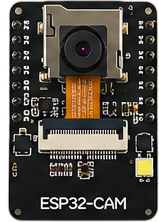
\includegraphics[height=2.6cm]{red_esp32cam.png}};
\draw[->, flecha, line width=1.3pt] ($(cam.west)+(0,0.1)$) -- ++(-0.9,0) |- ($(onx.south)+(-0.35,0.05)$);
\node[ip, below] at (cam.south) {192.168.4.50};

\node[tarjeta, anchor=west] at ($(cam.east)+(0.4,0)$) {%
  {\large\textbf{ESP32-CAM}}\\[4pt]
  \textbullet\ Estación Wi-Fi\\
  \textbullet\ IP fija\\
  \textbullet\ Stream de video};

\end{tikzpicture}
\end{document}
